\documentclass[tikz,border=3mm]{standalone}

% Inspired from https://davidstutz.de/illustrating-convolutional-neural-networks-in-latex-with-tikz/

\usepackage{amsmath}

\usetikzlibrary{decorations.pathreplacing}
\usetikzlibrary{fadings}
 
\begin{document}
 
	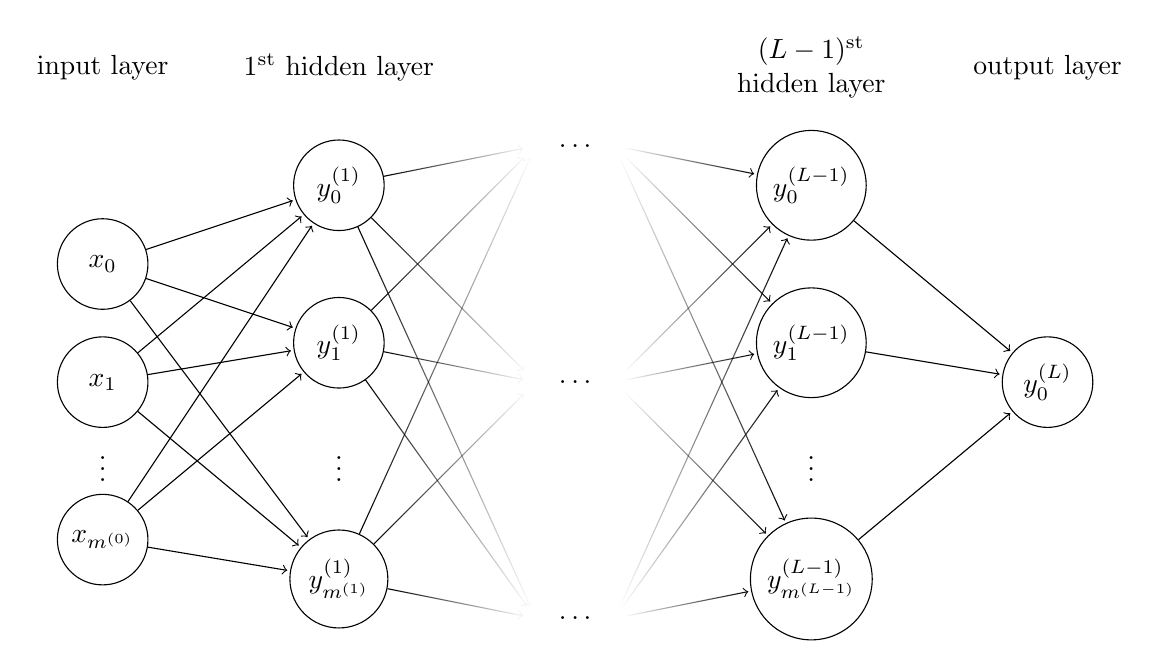
\begin{tikzpicture}[shorten >=1pt]
		\tikzstyle{node}=[draw,shape=circle,minimum size=1.15cm]
		
		% layer 0
		\node[node](x0) at (0,3.5){$x_0$};
		\node[node](x1) at (0,2){$x_1$};
		\node at (0,1){\vdots};
		\node[node](xm) at (0,0){$x_{m^{(0)}}$};

		% layer 1
		\node[node](h10) at (3,4.5){$y_0^{(1)}$};
		\node[node](h11) at (3,2.5){$y_1^{(1)}$};
		\node at (3,1){\vdots};
		\node[node](h1m) at (3,-0.5){$y_{m^{(1)}}^{(1)}$};
 
		% layer ...
		\node(h20) at (5.5,5){};
		\node(h21) at (5.5,2){};
		\node(h22) at (5.5,-1){};
		
		\node(d0) at (6,5){$\ldots$};
		\node(d1) at (6,2){$\ldots$};
		\node(d2) at (6,-1){$\ldots$};
 
		\node(hL10) at (6.5,5){};
		\node(hL11) at (6.5,2){};
		\node(hL12) at (6.5,-1){};
		
		% layer L-1
		\node[node](hL0) at (9,4.5){$y_0^{(L-1)}$};
		\node[node](hL1) at (9,2.5){$y_1^{(L-1)}$};
		\node at (9,1){\vdots};
		\node[node](hLm) at (9,-0.5){$y_{m^{(L-1)}}^{(L-1)}$};
		
		% layer L
		\node[node](y0) at (12,2){$y_0^{(L)}$};
		
		% 0 -> 1
		\draw[->] (x0) -- (h10);
		\draw[->] (x0) -- (h11);
		\draw[->] (x0) -- (h1m);
 
		\draw[->] (x1) -- (h10);
		\draw[->] (x1) -- (h11);
		\draw[->] (x1) -- (h1m);
 
		\draw[->] (xm) -- (h10);
		\draw[->] (xm) -- (h11);
		\draw[->] (xm) -- (h1m);
 
		% 1 -> ...
		\draw[->,path fading=east] (h10) -- (h20);
		\draw[->,path fading=east] (h10) -- (h21);
		\draw[->,path fading=east] (h10) -- (h22);
		\draw[->,path fading=east] (h11) -- (h20);
		\draw[->,path fading=east] (h11) -- (h21);
		\draw[->,path fading=east] (h11) -- (h22);
		\draw[->,path fading=east] (h1m) -- (h20);
		\draw[->,path fading=east] (h1m) -- (h21);
		\draw[->,path fading=east] (h1m) -- (h22);

		% ... -> L-1
		\draw[->,path fading=west] (hL10) -- (hL0);
		\draw[->,path fading=west] (hL11) -- (hL0);
		\draw[->,path fading=west] (hL12) -- (hL0);
		\draw[->,path fading=west] (hL10) -- (hL1);
		\draw[->,path fading=west] (hL11) -- (hL1);
		\draw[->,path fading=west] (hL12) -- (hL1);
		\draw[->,path fading=west] (hL10) -- (hLm);
		\draw[->,path fading=west] (hL11) -- (hLm);
		\draw[->,path fading=west] (hL12) -- (hLm);

		% L-1 -> L
		\draw[->] (hL0) -- (y0);
		\draw[->] (hL1) -- (y0);
		\draw[->] (hLm) -- (y0);

		% labels
		\draw (0,6) node {input layer};
		\draw (3,6) node {$1^{\text{st}}$ hidden layer};
		\draw (9,6) node [align=center] {$(L-1)^{\text{st}}$\\hidden layer};
		\draw (12,6) node [align=center] {output layer};
		%\draw [decorate,decoration={brace,amplitude=10pt},xshift=-4pt,yshift=0pt] (11.5,4) -- (12.75,4) node [black,midway,yshift=+0.6cm]{output layer};
	\end{tikzpicture}
 
\end{document}

